\documentclass[main.tex]{subfiles}
\pagenumbering{arabic}
\newcommand\chapterlabel{ChMIX-bond}\setcounter{figurenewcounter}{0}\setcounter{tablenewcounter}{0}\setcounter{formulanewcounter}{0}
\setcounter{chapter}{6}

\begin{document}



\chapter[Chemical bond ]{Chemical bond }

\begin{marginfigure}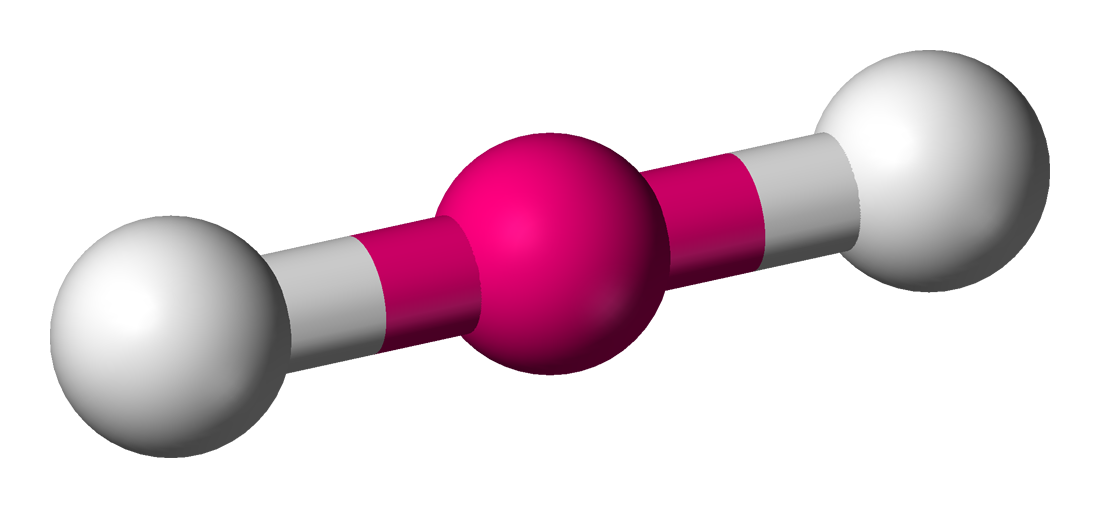
\includegraphics{../Ch-electronicstructure/figure1} \end{marginfigure}\import{../Ch-electronicstructure/files/}{ChapterIntro}

%\begin{marginfigure}%LEARNING GOALS BOX
%\begin{mytcbox}{GOALS}
%%
%\begin{center}\textcolor{blue}{\faEnvira Chemistry and molecules }\end{center}
%\begin{enumerate}[label=\protect\circled{\color{white}\arabic*}]
%  \import{../Ch-Gas/files/}{ChapterGoal-Ideal-gas-law}
%\end{enumerate}
%
%\begin{center}\textcolor{blue}{\faFlask Acids and bases }\end{center}
%\begin{enumerate}[label=\protect\circled{\color{white}\arabic*}]
%\import{../Ch-acidbase/files/}{SectionGoal-Blood-as-a-buffer-The-dangerous-change-in-blood-PH}
%\end{enumerate}
%
%\begin{center}\textcolor{blue}{\faTint  Electrolytes and solutions }\end{center}
%\begin{enumerate}[label=\protect\circled{\color{white}\arabic*}]
%\import{../Ch-Gas/files/}{ChapterGoal-Mixtures-of-gases}
%\end{enumerate}
%
%\begin{center}\textcolor{blue}{\faFire Reactions and energy} \end{center}
%\begin{enumerate}[label=\protect\circled{\color{white}\arabic*}]
% \import{../Ch-mole/files/}{SectionGoal-Chemical-reaction-Balancing-chemical-reactions}
%\end{enumerate}
%
%\begin{center}\textcolor{blue}{\faFlash The chemistry of cancer} \end{center}
%\begin{enumerate}[label=\protect\circled{\color{white}\arabic*}]
%\import{../Ch-nuclear/files/}{SectionGoal-Radioactive-gases:-radon}
%	\end{enumerate}
%	
%\begin{center}\textcolor{blue}{\faFlash Let's calculate} \end{center}
%\begin{enumerate}[label=\protect\circled{\color{white}\arabic*}]
%\import{../Ch-measurements/files/}{SectionGoal-Using-Conversion-Factors-Square-or-cubic-units}
%\import{../Ch-measurements/files/}{SectionGoal-Using-Conversion-Factors-Units-of-volume}
%\end{enumerate}
%			 				 
%
%
%
%
%\end{mytcbox}
%\vspace{1cm}
%%\begin{tcolorbox}[enhanced,colback=red!5!white,colframe=black!50!red,boxrule=1pt,
%%  arc=0pt,outer arc=0pt,drop heavy lifted shadow]
%%\faGears\ 
%% \import{../Ch-electrolytes/files/}{ChapterDiscussion}
%% \end{tcolorbox}
%\end{marginfigure}%LEARNING GOALS BOX






\renewcommand\chapterlabel{Ch-electronicstructure}

\section{Electron-dot structures of atoms}\import{../\chapterlabel/files/}{SectionIntro-Electron-dot-structures-of-atoms}
\sloppy\begin{description}
\item[\docfilehook{Valence electrons}{}] \import{../\chapterlabel/files/}{SubSection-Electron-dot-structures-of-atoms-Valence-electrons}
\import{../\chapterlabel/problems/}{SampleProblem1}
\item[\docfilehook{The octet rule}{}] \import{../\chapterlabel/files/}{SubSection-Electron-dot-structures-of-atoms-The-octet-rule}
\item[\docfilehook{Electron-dot structure of an atom}{}] \import{../\chapterlabel/files/}{SubSection-Electron-dot-structures-of-atoms-Electron-dot-structure-of-an-atom}
\import{../\chapterlabel/problems/}{SampleProblem2}
\item[\docfilehook{Electron-dot structure of diatomic molecules}{}] \import{../\chapterlabel/files/}{SubSection-Electron-dot-structures-of-atoms-Electron-dot-structure-of-diatomic-molecules}
\import{../\chapterlabel/problems/}{SampleProblem3}
\item[\docfilehook{Electron-dot structure of general molecules}{}] \import{../\chapterlabel/files/}{SubSection-Electron-dot-structures-of-atoms-Electron-dot-structure-of-general-molecules}
\import{../\chapterlabel/problems/}{SampleProblem4}
\item[\docfilehook{Atomic charges in a molecule}{}] \import{../\chapterlabel/files/}{SubSection-Electron-dot-structures-of-atoms-Atomic-charges-in-a-molecule}
\import{../\chapterlabel/problems/}{SampleProblem5}
\item[\docfilehook{Multiple bonds}{}] \import{../\chapterlabel/files/}{SubSection-Electron-dot-structures-of-atoms-Multiple-bonds} 
\import{../\chapterlabel/problems/}{SampleProblem6}
\end{description}
\section{Molecular shape}\import{../\chapterlabel/files/}{SectionIntro-Molecular-shape}
\sloppy\begin{description}
\item[\docfilehook{ABE Molecular code}{}] \import{../\chapterlabel/files/}{SubSection-Molecular-shape-ABE-Molecular-code}
\newpage\vspace{5cm}\import{../\chapterlabel/files/}{Table-Molecular-geometries}
\import{../\chapterlabel/problems/}{SampleProblem7}
\end{description}
\section{Polarity of molecules}\import{../\chapterlabel/files/}{SectionIntro-Polarity-of-molecules}
\sloppy \begin{description}
\item[\docfilehook{Bond polarity}{}] \import{../\chapterlabel/files/}{SubSection-Polarity-of-molecules-Bond-polarity}
\item[\docfilehook{Polarity of diatomic molecules}{}] \import{../\chapterlabel/files/}{SubSection-Polarity-of-molecules-Polarity-of-diatomic-molecules}
\import{../\chapterlabel/files/}{SubSection-Polarity-of-molecules-Molecules-with-the-same-polarity}
\item[\docfilehook{Polarity of larger molecules}{}] \import{../\chapterlabel/files/}{SubSection-Polarity-of-molecules-Polarity-of-larger-molecules}
\import{../\chapterlabel/problems/}{SampleProblem8}
\item[\docfilehook{Polarity and mixing}{}] \import{../\chapterlabel/files/}{SubSection-Polarity-of-molecules-Polarity-and-mixing}
\item[\docfilehook{Molecules with the same polarity}{}] \import{../\chapterlabel/files/}{SubSection-Polarity-of-molecules-Molecules-with-the-same-polarity}
\item[\docfilehook{Molecules with different polarity}{}] \import{../\chapterlabel/files/}{SubSection-Polarity-of-molecules-Molecules-with-different-polarity}
\end{description}




\end{document}
 
